\chapter{Marco teórico}
\label{ch:marco}
\subsection*{Diseño de ASICs}

%{Esta tesis no pretende exponer el proceso de fabricación de un circuito integrado, esa información puede encontrarse en un libro de texto sobre diseño VLSI; sin embargo, en las secciones siguientes se expondrá brevemente, la metodología que se esta usando para que a futuro se pueda llevar a cabo la implementación de un sistema sobre un dado de silicio (silicon dice), entendiendo por dado el espacio que el sistema propuesto ocupará sobre la oblea de silicio, al final del proceso de fabricación.
%
%Comercialmente la manufacturación de ASICs no es rentable para aplicaciones de envergadura pequeña, ya que un proceso de fabricación fácilmente alcanza los millones de dolares, si se tiene una proyección comercial baja o nula esta opción queda descartada, la forma más fácil de implementar un diseño en un chip sería venderle la idea o diseño a un fabricante.
%
%No obstante, venderle la idea o diseño a un fabricante implica revelar información sensible sobre el producto y el fabricante probablemente este trabajando con su competencia por lo que revelarle su trabajo a un fabricante tampoco es la mejor opción.
%
%Sin embargo, es posible hacer el proceso de diseño, posteriormente generar un archivo que contenga toda la información estrictamente necesaria para que el fabricante pueda implementar el diseño sobre el chip, sin tener revelar la información sensible que se pretende proteger.
%
%Esta suele ser la opción más viable para los pequeños investigadores; no obstante, existe la problemática que este tipo de servicio alcanza precios muy elevados sobre todo si se pretende emplear los procesos más modernos y las tecnologías de vanguardia.
%
%En respuesta a la problemática de no tener suficientes fondos para concretar una fabricación, existe el servicio de óbleas multiproposito de la universidad de Berkeley (\textit{MOSIS}).
%
%La funcionalidad de implementar sistemas sobre chips (SoC) tiene grandes ventajas respecto a sistemas embebidos o implementados mediante software de alto nivel.

Este trabajo no pretende exponer el proceso de fabricación de un circuito integrado. En las secciones siguientes se expondrá brevemente, la metodología usanda para que a futuro se pueda llevar a cabo la implementación de un sistema sobre un dado de silicio \footnote{Entendiendo por dado el espacio que el sistema propuesto ocupará sobre la oblea de silicio, al final del proceso de fabricación} (silicon dice), usando las herramientas de Synopsys.

En primera instancia producir un sistema en un circuito integrado representa una mejor protección para los derechos intelectuales, pues su contenido difícilmente es reproducible. Un circuito integrado presenta enormes facilidades de portabilidad debido a su tamaño y su consumo energético. Lo cual es el principal objetivo del proyecto: "Sonidos Ilegales".

%\subsection*{Sobre la tecnología de fabricación}
%
%Para el presente proyecto se hace uso de la tecnología de IBM CMOS8RF (CMRF8SF), esta tecnología cuenta con una alta densidad de lógica CMOS de  0.13 $\mu$m destinada a aplicaciones de señal mixta, en ámbitos asociados al procesamiento analógico y de radio frecuencia . Entre las generalidades del proceso, cabe destacar que cuenta con 8 capas de metal, y la tensión $V_{DD}$ de los dispositivos se encuentra en un rango de 1.2 V a 1.5 V.\\

\section{Tipos de diseño circuitos integrados digitales}

La clasificación del diseño de circuitos integrados se puede apreciar en el esquema de la figura \ref{ICs}.

\begin{figure}[h]
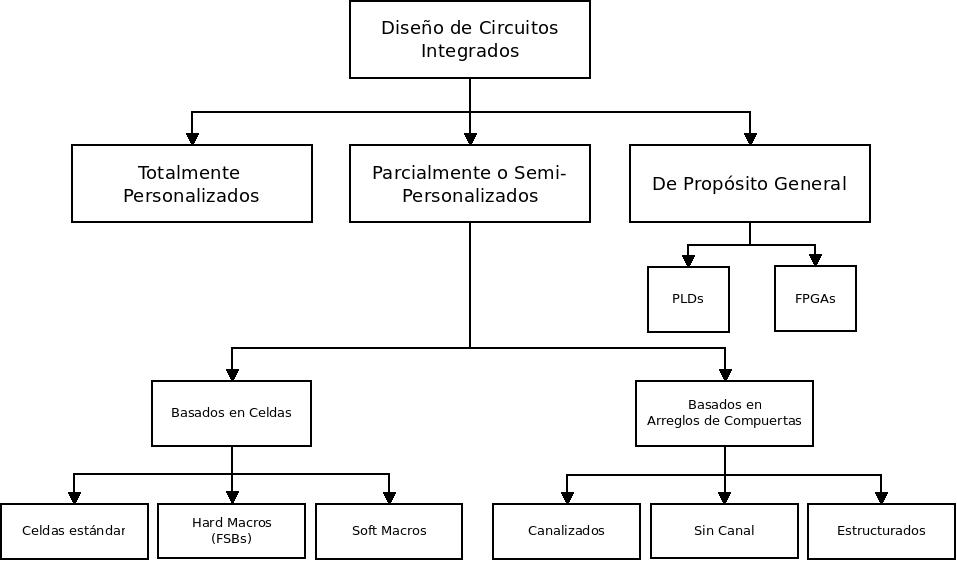
\includegraphics[width=\textwidth]{Tipos_de_ICs.jpeg}
\centering
\caption{Tipos de Diseño de Circuitos Integrados}
\label{ICs}
\end{figure}
Como puede observarse el diseño de circuitos integrados (de aquí en adelante ICs\footnote{ICs: acrónimo en inglés para circuitos integrados}) se puede clasificar a grosso modo en tres tipos principales:

\subsection{\textbf{ICs totalmente personalizados}}

En esta metodología de trabajo los diseñadores generan todas las celdas lógicas de acuerdo con las necesidades tiene el diseño que se pretende realizar, lo que contempla la concepción funcional, lógica y física de cada celda. También se desarrollan las máscaras necesarias para la fabricación del chip sobre la oblea de silicio.

Empresas como Intel son un buen ejemplo de industrias dedicadas al desarrollo de circuitos integrados totalmente personalizados. Aquí los ingenieros invierten enormes cantidades de tiempo maximizando el aprovechamiento de cada micrómetro cuadrado disponible en el dado, lo que les permite incluir circuitos analógicos, optimizar celdas de memoria e incluso contemplar y mejorar la eficiencia mecánica de las estructuras de conexión y ubicación de los componentes del chip.

Esta es la metodología más costosa de todas, no obstante, es la respuesta adecuada si el diseñador necesita de unidades (celdas) más eficientes en términos energéticos y velocidad, de las que es capaz de encontrar en una biblioteca de celdas existentes. Es comúnmente utilizada por empresas dedicadas a la innovación y el desarrollo tecnológico.

\subsection{\textbf{ICs programables}}

Estos consisten en dispositivos lógicos programables (PLDs), que son circuitos integrados con configuraciones estándar predeterminadas. Algunos ASICs para permiten la personalización de algunas funciones puntuales, por lo que aunque sean estructuras prediseñadas y flexibles, son consideradas como una rama del diseño de ICs.

\subsection{\textbf{ICs semipersonalizados}}

Son aquellos ICs para los cuales existe una biblioteca de celdas estándar y posiblemente todas las mascaras de diseño están disponibles. El uso de bibliotecas de celdas prediseñadas hace el diseño más fácil. Está metodología de diseño se subdivide en dos partes:

\subsubsection{Basado en arreglos de compuertas}

En este tipo de diseño los transistores se encuentran predefinidos en un patrón dado sobre en la oblea de silicio. Este patrón se conoce como arreglo base y a los elementos más pequeños se los conoce como celdas base o celdas primitivas.

En esta técnica el diseñador únicamente define la interconexión de las celdas usando para ello máscaras personalizadas. Así el diseñador escoge de entre una basta biblioteca de celdas prediseñadas y precaracterizadas. Las celdas lógicas suelen ser denominadas como macros. La razón de esto se debe a que el trazado de la celda base es el mismo para cada celda lógica y únicamente se personaliza la interconexión y el enrutado dentro de las celdas y con las celdas adyacentes, de manera similar a un macro de software.

Existen subcategorías del uso de esta técnica, pero esa información excede el alcance de esta tesis, por lo que no serán expuestas. Se invita al lector a considerar una bibliografía pertinente \cite{book:johnM1997,book:barrK2006}

\subsubsection{Basado en celdas estándar}

Un circuito integrado basado en celdas estándar usa celdas lógicas prediseñadas como compuertas ``Y", ``O", ``Flip Flops", ``Multiplexores", etc.. Estas celdas se conocen como celdas estándar.

Suele usarse el término \textit{CBIC} para esta categoría. El área de ubicación de las celdas estándar en un \textit{CBIC} se construye en hileras, de manera similar a una pared de ladrillos. Las celdas estándar pueden y suelen ser utilizadas en conjunto a microcontroladores, o microprocesadores, conocidos como ``Mega celdas". Este término también se emplea para bloques totalmente personalizados, y suelen ser denominados como: ``Macros a Nivel de Sistema (SLMs)", ``Mega Funciones", ``Bloques Fijos", o ``Bloques Funcionales Estándar (FSBs)".

En esta metodología es diseñador define únicamente la colocación y el enrutado (interconexión entre celdas estándar) de las celdas estándar; sin embargo, estás pueden ser colocadas libremente en el área disponible del dado. Esto implica que las máscaras de fabricación en un \textit{CBIC} son únicas para cada cliente.

Usar \textit{CBICs} tiene enormes ventajas ya que permite hacer diseños más flexibles y optimizarlos en términos de aprovechamiento de área, velocidad o consumo energético. Adicionalmente las bibliotecas de celdas estándar suelen ofrecer las mismas celdas estándar prediseñadas para cumplir distintas las expectativas de desempeño, enfocadas a tamaño, velocidad o energía.

Las principales desventajas consisten en que el tiempo necesario para el diseño suele ser elevado, debe comprarse una biblioteca de celdas estándar, y se está sujeto a las restricciones de ésta, y finalmente las máscaras de fabricación serán nuevas con cada nuevo diseño o versión de diseño, lo cual implica tiempo adicional, además de costos adicionales por parte del fabricante.

La información de esta sección se tomó a partir de las fuentes \cite{book:raj2008,book:johnM1997,book:raj2008}

\section{Flujo de diseño digital para el diseño de circuitos integrados digitales}

Dada la complejidad en el proceso de diseño de circuitos integrados, es imperativo llevar a cabo un diseño estructurado, que use los principios de jerarquización, modularidad, regularidad y localidad para manejar la complejidad del diseño.

El diseño digital VLSI suele ser particionado en cinco niveles de abstracción: diseño de arquitecturas, diseño de microarquitecturas, diseño lógico, diseño de circuitos y diseño físico. Estas etapas son ejecutadas en paralelo, y en muchas ocasiones son depedientes entre si.

Una manera alternativa de analizar el diseño estructurado es mediante el ``diagrama Y" mostrado en la figura \ref{Ychart}. 

\begin{figure}[h]
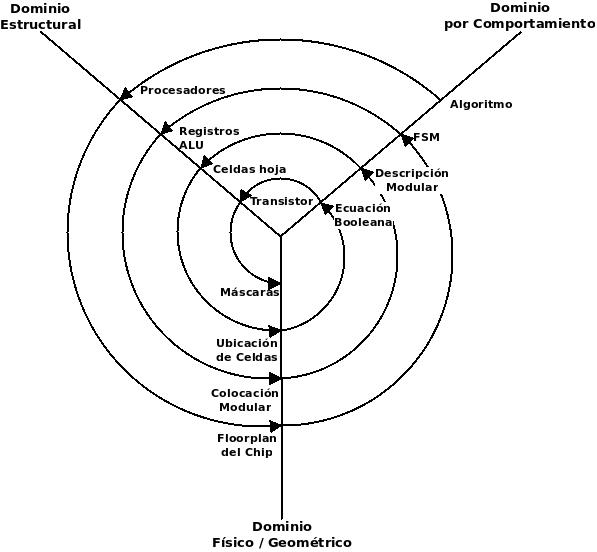
\includegraphics[width=\textwidth]{Gajski_Y_Chart.jpeg}
\centering
\caption{Diagrama de Gajski. Espiral que ilustra el flujo digital de diseño de circuitos integrados y cuyas arístas establecen los ámbitos por los que debe atravesar el diseño. Figura de autoría propia basada en lo expuesto en la sección 1.6 del libro: CMOS VLSI Design, Weste, Harris.}
\label{Ychart}
\end{figure}


El diagrama de Gajski o diagrama Y, permite entender el concepto de abstracción en el diseño digital, pues se parte desde un concepto general de diseño y al interiorizar en el diagrama se desvelan las etapas que llevan hasta la fabricación correcta del circuito integrado.

%El dominio por comportamiento describe qué hace el sistema, seguidamente en el dominio estructural, el cual expone la interconexión de los módulos capaces de realizar el comportamiento deseado, eventualmente a los niveles de abstracción más bajos donde se describen las compuertas individuales y las conexiones entre los transistores que las componen. Finalmente en cada nivel de abstracción del dominio físico se explica como se construye físicamente ese nivel de abstracción, en los niveles más altos se considera el diseño del floorplan del chip, donde en esencia se , y consecuentemente al internarse en los niveles más profundos se describen la geometría actual de cada transistor individual.

El proceso de diseño puede verse como la transformación desde un dominio hacia otro manteniendo la equivalencia de los dominios. Las descripciones por comportamiento se transforman en descripciones estructurales y estas a su vez son transformadas en descripciones físicas. Cada transformación es validada, ya sea manualmente o mediante herramientas automatizadas. La especificación jerárquica de cada dominio y sucesivamente detallando sus niveles de abstracción es lo que permite diseñar grandes sistemas. 

La razón para describir en detalle los niveles de abstracción y los respectivos dominios es para definir un proceso de diseño en el cual la función final del sistema es capaz de rastrearse hasta la descripción por comportamiento inicial.

El diagrama Y muestra las transformaciones entre cada dominio y las variaciones entre los niveles de abstracción. El flujo de diseño procede desde los anillos exteriores hacia los interiores, profundizando en niveles de abstracción cada vez más complejos, de acuerdo a una jerarquía establecida.

Para más detalles ir a la sección 1.6 de \cite{book:weste2005}.

\subsection{Generalidades del flujo de diseño digital}
\label{sec:gen_d_flow}
\begin{figure}[t]
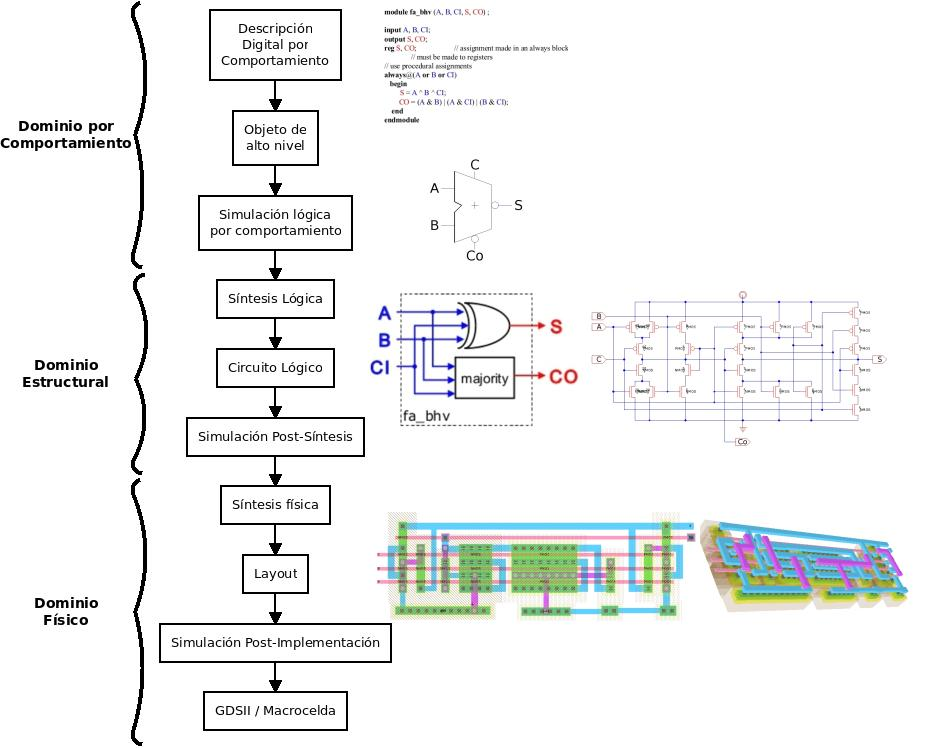
\includegraphics[width=\textwidth]{Flujo_Digital.jpeg}
\centering
\caption{Esquema representativo e ilustrativo del flujo de diseño de circuitos integrados digitales}
\label{Dflow1}
\end{figure}

Como se mencionó en el apartado anterior, el diseño comienza a dar sus pasos en cuanto es concebida una función o proceso y su comportamiento ha sido modelada en un algoritmo, ya sea secuencial, concurrente o una mezcla de ambos. Este algoritmo se traduce a un lenguaje estandarizado, el cual en el caso de los circuitos integrados digitales corresponde a un \textit{HDL}, que en términos concretos es la descripción digital del circuito integrado o el modelo digital.

Partiendo del modelo digital se puede hacer una verificación de comportamiento, que en términos técnicos se denomina simulación lógica. El modelo digital no es más que un objeto de alto nivel capaz de emular el comportamiento deseado. Su utilidad es poca para el diseñador, ya que no provee datos sobre el desempeño del diseño, únicamente provee 
información a nivel de comportamiento; sin embargo, es el punto de partida en el flujo de diseño.

Una vez que la simulación lógica es satisfactoria, se procede a usar el modelo por comportamiento y asociar los módulos descritos en él, con unidades lógicas provistas de características de retardos (sincronización de señales), consumo energético, y área, las cuales se encuentran en la biblioteca de la tecnología que se usará en la fabricación. A este proceso se le conoce como síntesis lógica, y genera una base de datos que contiene datos de las celdas estándar y las conexiones entre ellas para ejecutar las funciones abstraídas del modelo de comportamiento.

La base de datos creada en el proceso de síntesis permite generar un nuevo modelo codificado en HDL y una primera aproximación del desempeño de los módulos diseñados, i.e. un modelo con la información sobre los retardos de propagación de las señales en las celdas y entre las mismas, un presupuesto de la energía disipada y el área necesaria para ubicar las celdas usadas. Este nuevo modelo, denominado como modelo post-síntesis nuevamente se simula con el mismo arreglo o banco de pruebas usado en la simulación por comportamiento.

La simulación post-síntesis permite observar el retardo de propagación de las señales, y confirmar si las expectativas de sincronización son alcanzadas. También permite verificar si los datos son generados en los plazos necesarios, y poder garantizar una funcionalidad correcta de los módulos y el diseño en lo concerniente al desempeño de las celdas estándar. 

Cuando los resultados obtenidos en la síntesis lógica y la simulación respectiva sean satisfactorios, se toma el modelo post-síntesis y se usa esta información para empezar con el plano de piso (floorplan) del chip. Las celdas estándar son invocadas a un área determinada, y posteriormente se establecen las conexiones que permiten implementar los módulos abstraídos en la primera etapa del diseño (el modelo de comportamiento). Este proceso recibe el nombre de síntesis física o implementación física, ()en esta tésis se usará la palabra síntesis para referirse a la síntesis lógica, y la palabra implementación será usada para referirse a la síntesis física).

Posteriormente, se genera una nueva base de datos con información más precisa sobre el diseño. Retardos debido a efectos parasíticos, distancia del recorrido de las señales, perdidas resistivas del alambrado, y otros efectos que serán expuestos más adelante.

Nuevamente se genera una base de datos con la información del colocamiento y el enrutado (\textit{Place\&Route}), que incluye modelos más de sincronía y potencia más completos, y otra representación HDL del diseño post implementación. Esta etapa permite obtener una respuesta más precisa de diseño. Al igual que en la etapa anterior, se crean reportes de consumo energético, aprovechamiento de área, calidad de resultados (QOR, que es un compendio de la información más relevante de todos los reportes generados), etc.

Cuando una simulación post-implementación es satisfactoria se procede a dar por concluido el flujo, y a continuación se establecen dos panoramas.

En el primer caso nuestro diseño está completo por lo que se procede a compilar la base de datos en un archivo estándar para condensar la información necesaria para el fabricante. Aquí se valora si el diseño tiene probabilidad alta de ser fabricado con éxito, siendo así la información suministrada será usada para desarrollar las máscaras necesarias para la construcción del chip.

El segundo escenario consiste en que el diseño en el que se ha estado trabajando no es el producto final, sino que forma parte de otro diseño más complejo y grande, el cual aún no se haya terminado. En ese caso la base de datos servirá para generar una macro celda que será utilizada en diseños posteriores.

En la figura \ref{Dflow1} se aprecia un resumen gráfico de la explicación anterior.

\subsection{Flujo de diseño digital en las herramientas de Synopsys}

Synopsys es una empresa que brinda herramientas de diseño asistido por computadora (CAD), para la automatización de procesos en el diseño de circuitos integrados. El flujo de diseño digital suele ser similar independientemente del proveedor de las herramientas; sin embargo, esta tesis gira entorno a los softwares de Synopsys, por lo que se expondrá la metodología de diseño usando este proveedor.

\subsection{Front End}

\begin{figure}[h]
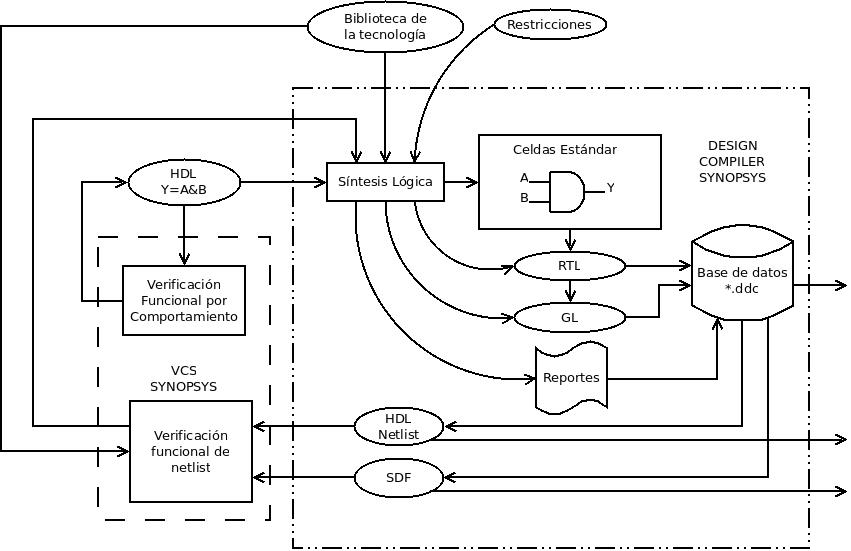
\includegraphics[width=\textwidth]{Front_End.jpeg}
\centering
\caption{Esquema ilustrativo del flujo de diseño de circuitos integrados digitales, enfocado a las herramientas de síntesis lógica, en esencia las herramientas de Front End}
\label{fe}
\end{figure}


El término "Front End", es un concepto en inglés asociado a la jerga del desarrollo de software, y significa interfaz; sin embargo, en el caso del diseño de circuitos integrados, no se generan softwares y tampoco interfaces. Una traducción más literal, y por lo tanto, menos elegante del concepto sería "Fachada", y es en esencia con lo que el diseñador interactúa en la primer etapa del diseño.

Al decir que el diseñador interactúa con una fachada, se debe entender que el diseñador trabaja con el cascarón de un elemento que intrínsecamente no es circuito electrónico como tal, si no un modelo abstracto que presenta un comportamiento de causa efecto, el cual, naturalmente, es acorde a la semántica de la lógica digital, o lógica binaria. Recurriendo nuevamente a la jerga del software, podemos entender el front end o fachada como aquello relacionado con un objeto de alto nivel, que ofrece un vector de respuestas de acuerdo con la dinámica de un vector de estímulos.

El diseñador comienza a acercarse al diseño del circuito integrado, considerando y definiendo los aspectos principales de la fachada. Retomando el diagrama de Gajski (figura \ref{Ychart}), el proceso de "Front-End" consiste en la transición del modelo de comportamiento a un modelo estructurado, que se asocia con las funciones de las celdas estándar ofrecidas por la tecnología y el fabricante.

Condensando lo anterior, las herramientas de "Front-End" de un proveedor, son aquellas que ejecutan o facilitan el proceso de síntesis lógica en el flujo digital del diseño de circuitos integrados. En el caso de "Synopsys", estas herramientas son principalmente "Design Compiler" y "VCS", existen otras herramientas adicionales asociadas a la familia de "Design Compiler", "VCS" y el "Shell" de "Design Compiler" son las principales y suelen ser suficientes.

En la figura \ref{fe} se aprecia un diagrama que ilustra como el proceso expuesto en la sección \ref{sec:gen_d_flow}, es implementado por las herramientas de "Synopsys" todos los procesos en el diseño de circuitos integrados tienen un componente iterativo, y en este diagrama vemos como antes de avanzar en el flujo, se atraviesa por etapas a las que se recurre con frecuencia, estas etapas son las simulaciones por comportamiento y post-síntesis. La depuración de la etapa de síntesis es esencial para garantizar el éxito final del proyecto, por lo que las simulaciones tienen una gran importancia.

Cómo se observa desde el diagrama de Gajski (figura \ref{Ychart}), las herramientas de "front end" traducen el diseño por comportamiento en modelos de altos nivel de circuitos digitales, aunque como tal no se trabajan con circuitos lógicos reales, y para efectos prácticos el diseñador nunca trabaja realmente con elementos lógicos y digitales, las herramientas proveen la virtualización del comportamiento diseñado, mediante una biblioteca de simulación, las celdas estándar abstraídas en el proceso de síntesis, se comportarán como un elemento de circuito digital real, de ahí que se pueda validar si la etapa de síntesis cumple las expectativas del diseñador.

\newpage
\subsection{Back End}

\begin{figure}[h]
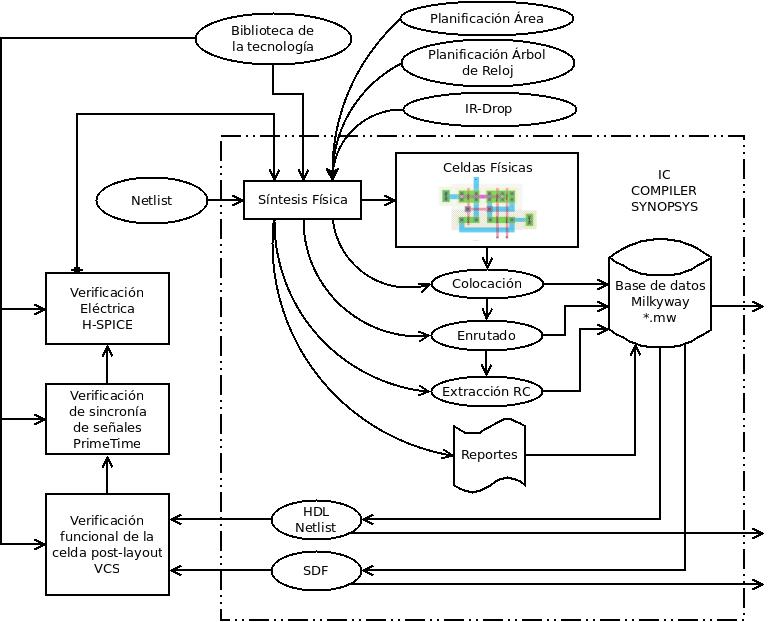
\includegraphics[width=\textwidth]{Back_End.jpeg}
\centering
\caption{Esquema ilustrativo del flujo de diseño de circuitos integrados digitales, enfocado a las herramientas de síntesis lógica, en esencia las herramientas de Front End}
\label{be}
\end{figure}

Se refiere a aquellos procedimientos relacionados con la constitución interna de un proyecto, nuevamente se emplea el anglicismo "Back End" para referirse a dichos procesos. No existe un concepto en español capaz de traducir el significado de esta palabra, pero se podría entender como todos aquellos aspectos ocultos al macro diseñador, entendiendo por oculto, una serie de elementos compuestos por elementos más simples hasta llegar a las unidades fundamentales de la electrónica moderna, i.e. transistores. Una analogía curiosa, y que ilustra bien esta situación es la de la muñeca matryoshka \cite{book:matryoshka}, cada muñeca contiene a otra muñeca más pequeña, y se interioriza así hasta alcanzar una pequeña muñeca que no contiene a ninguna otra.

En el proceso de diseño de circuitos integrados, semipersonalizados, y basados en celdas estándar, el diseñador no alcanza a trabajar directamente con transistores, o con los elementos que componen las celdas, si no, que da por hecho que las celdas estándar son funcionales y parte de ellas para generar nuevas macroceldas, y con las cuales se ejecutarán las funciones establecidas por el macromodelado del funcionamento del diseño.

En síntesis de lo anterior, el diseñador de "back end" trabaja con las etapas ocultas para los diseñadores de comportamiento, y síntesis del diseño, dónde los primeros establecen la semántica del diseño, y los segundos generan cajas negras que realizan las funciones descritas por sus antecesores, estas cajas negras manifiestan el comportamiento de una unidad electrónica real, en términos de consumo energético, área, y tiempos de propagación de señales, pero no dejan de ser modelos de alto nivel que no son circuitos electrónicos como tales, y es por ello que ha esta etapa se le denomina fachada.

En el proceso de "back end" las cajas negras abstraídas en el proceso de síntesis adquieren información más realista y equivalente a la de una celda física real. Esto podemos apreciarlo en la figura \ref{Dflow1} en el extremo derecho de la figura vemos como se muestran las etapas del flujo, en el dominio estructural, donde operan las herramientas de síntesis, aquí se muestran los bloques funcionales a nivel lógico. Al descender en el flujo expuesto en la misma figura, observamos la celda estándar que se abstrae del diseño estructurado, y su layout o implementación física, donde se aprecian los metales que interconectan las celdas y los transistores que componen las celdas.

Las herramientas de "back end" se encargan de facilitar el colocado y enrutado de las celdas estándar que se abstrajeron de la síntesis lógica. En el "back end" se asocia la base de datos post síntesis con la base de datos de la tecnología, invocando celdas físicas para generar un nuevo layout que implemente el diseño sintetizado. "Synopsys" cuenta con una herramienta llamada "IC Compiler", este software le permite al diseñador establecer los criterios de optimización del layout en términos de aprovechamiento de área, colocación selectiva para mejorar la eficiencia del consumo energético, sincronización de señales críticas, como lo es una señal de reloj, definir criterios de alambrado (enrutado) para sopesar las pérdidas resistivas, controlar fenómenos de electromigración y radiación o antena.




